\chapter{Supplementary Results and Corpus Data}
\label{sec:results}
The averages for each search method over their successful programs for each implementation are given in \cref{fig:SearchPerformance}. Note that each method succeeds on \textit{differing} sets of programs.

\begin{figure}
  \centering
  \begin{tabular}{lc|cccc}
  & Averages & \multicolumn{4}{c}{\textbf{Implementations}}\\
   & unit & \texttt{DFS} & \texttt{BDFS} & \texttt{IDFS} & \texttt{BFS}\\
   \hline
   \textbf{Time} & ms &  7.6 & 73 & 140 & 120\\
   \textbf{Major Heap} & mB & 3.7 & 32 & 5.9 & 25\\
   \textbf{Minor Heap} & mB & 66 & 680 & 1900 & 1300
  \end{tabular}
  
\caption{Benchmarks: Search Implementations}
\label{fig:SearchPerformance}
\end{figure}


Cast are between slices `from' a type `to' a type. Their average sizes given in \cref{fig:CastSlicingEffectiveness}.

\begin{figure}[h]
  \centering
  \begin{tabular}{lc|cc|cc}
  \multicolumn{2}{c}{\textbf{Averages}} & \multicolumn{4}{c}{\textbf{Subdivisions}}\\
  & & \multicolumn{2}{c|}{\textbf{Ok}} & \multicolumn{2}{c}{\textbf{Errors}}\\ 
   & unit & from & to & from & to\\
   \hline
   \textbf{Cast Slice} & size &  5.5 & 1.2 & 5.9 & 1.5 \\
   Std. dev. &  				 &  8.1 & 3.7 & 7.1 & 2.0\\
   \textbf{Proportion}& \%    & 1 & 0.2 & 1 & 0.2\\
   Std. dev. &  				 &  1 & 0.5 & 1 & 0.4\\
   \multicolumn{6}{c}{\textit{(Unannotated)}}\\
   \textbf{Type Slice} & size &  4.8 & 6.3 & 6.9 & 4.4  \\
   Std. dev. 			&    &  11 & 13 & 9.1 & 9.3\\
   \textbf{Proportion}& \% 	 & 1 & 2 & 2 & 1\\
   Std. dev. &  				 &  1 & 1 & 1 & 1\\
   \multicolumn{6}{c}{\textit{(Annotated)}}
  \end{tabular}
  \caption{Effectiveness: Cast Slices}
\label{fig:CastSlicingEffectiveness}
\end{figure}

Trace length and instantiation size data in \cref{fig:WitnessSize}.
\begin{figure}[h]\centering
\begin{tabular}{l|cccc}
& DFS & BDFS & BFS & IDFS\\
\hline
\textbf{Witness Size} Avg. & 1.1& 1.9&1.4&  2\\
Std. dev. & 1.2& 2.3&1.4&  2.3\\
\textbf{Trace size} Avg. & 33& 32& 11& 17\\
Std. dev. & 35& 33&2.4& 5
\end{tabular}
\caption{Witness \& Trace Sizes}
\label{fig:WitnessSize}
\end{figure}

Some examples of programs in the translated corpus are given in \cref{fig:}. All three were examples where BDFS did not terminate, and are accompanied with their failure classification.

\begin{figure}
\centering
\begin{subfigure}{1\textwidth}
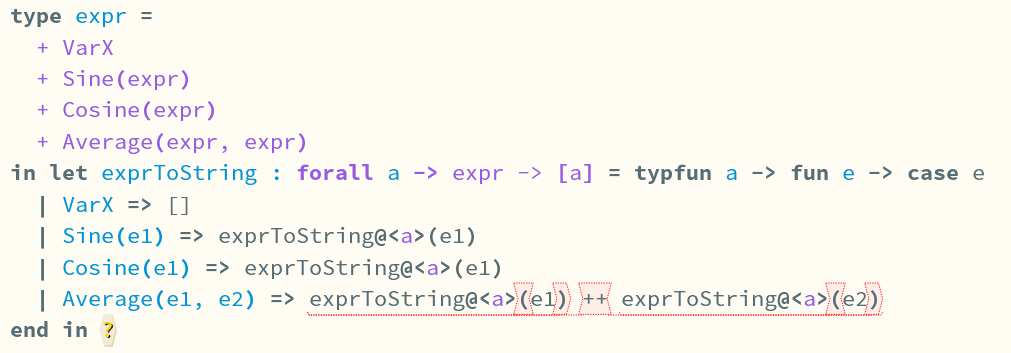
\includegraphics[width=1\textwidth]{Media/Figures/witness_exists}

Depth-first bias caused the procedure to try mostly permutations of \code{Sine(...)} and \code{Cosine(...)}. The error was on the \code{Average(...)} branch, not found within the time limit.
\caption{Witness Exists: prog2270.typed.hazel}
\end{subfigure}

\begin{subfigure}{1\textwidth}
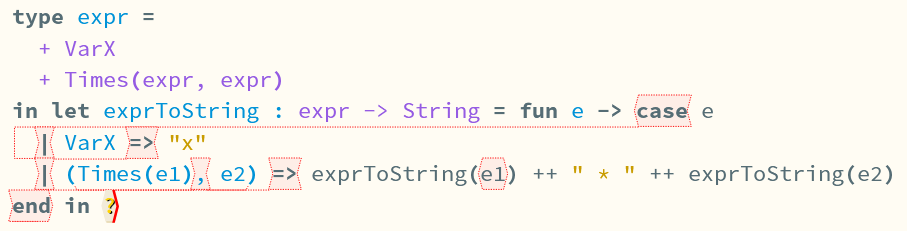
\includegraphics[width=0.8\textwidth]{Media/Figures/dead_code_pattern_instantiation}

A tuple pattern is used when an \code{expr} is expected. Instantiation only tries value of type \code{expr}. Further, another error exists inside this inaccessible branch.
\caption{Dead Code -- Wildcard: prog0080.typed.hazel}
\end{subfigure}

\begin{subfigure}{0.7\textwidth}
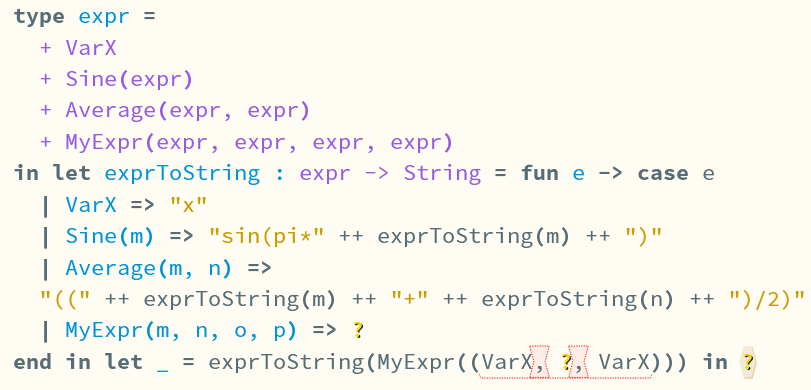
\includegraphics[width=1\textwidth]{Media/Figures/dead_code_wildcard}
Product arity inconsistency is present in inaccessible code bound to the wildcard pattern.
\caption{Dead Code -- Pattern Cast Failure: prog0339.typed.hazel}
\end{subfigure}
\caption{(Paraphrased) Failure Examples}
\label{fig:FailureExamples}
\end{figure}